\documentclass[a4paper,10pt]{article}
\usepackage[lmargin=2.0cm, rmargin=1.0cm,tmargin=3.5cm,bmargin=1.5cm]{geometry}
\usepackage{color,graphics}
\usepackage[export]{adjustbox}
\usepackage{lipsum}

\usepackage{graphicx}

\usepackage{listings}
\usepackage[scaled=0.75]{helvet}

\begin{document}
\setcounter{secnumdepth}{-1} 

\begin{center}
\textbf{\LARGE Installation and Configuration of Oracle Virtual Box}
\end{center}

\raggedright Expt No: 1 \hfill \raggedleft Feburary 20, 2019 \\ 

\raggedright Author: Subalakshmi Shanthosi S  (186001008) \par 

\noindent\makebox[\linewidth]{\rule{\textwidth}{1pt}} 

\section{Aim}
To configure and install Oracle Virtual Box in Ubuntu 18.04 LTS OS flavour.

\section{Software's Used}
\begin{itemize}
  \item Oracle VirtualBox
\end{itemize}

\section{Description}
Installation of Oracle VirtualBox with guest Operating System as Ubuntu 16.04.Installation of neccessary packages namely - openssh-server,openssh-client,java in the created virtualbox instance.
\section{Procedure}

\begin{enumerate}
	\item Install Oracle VirtualBox using apt-get command.
	\item Choose guest Operating System as Ubuntu 16.04 LTS and architecture as x86.
	\item Set your base RAM memory above 2 GB.
	\item Create a virtual hard disk drive and select dynamically allocated space.
	\item Erase and install the OS from the iso disk image of Ubuntu 16.04 LTS.
	\item Let the installation of all required packages complete.
	\item Create a guest OS user with valid credentials.
	\item Login to the created virtualbox instance and install the following packages using apt-get command
	\begin{itemize}
		\item openssh-server
		\item openssh-client
		\item java jdk 7
		\item javac compiler
	\end{itemize}
\pagebreak
\end{enumerate}

\section{Output}

\begin{figure}[h]
	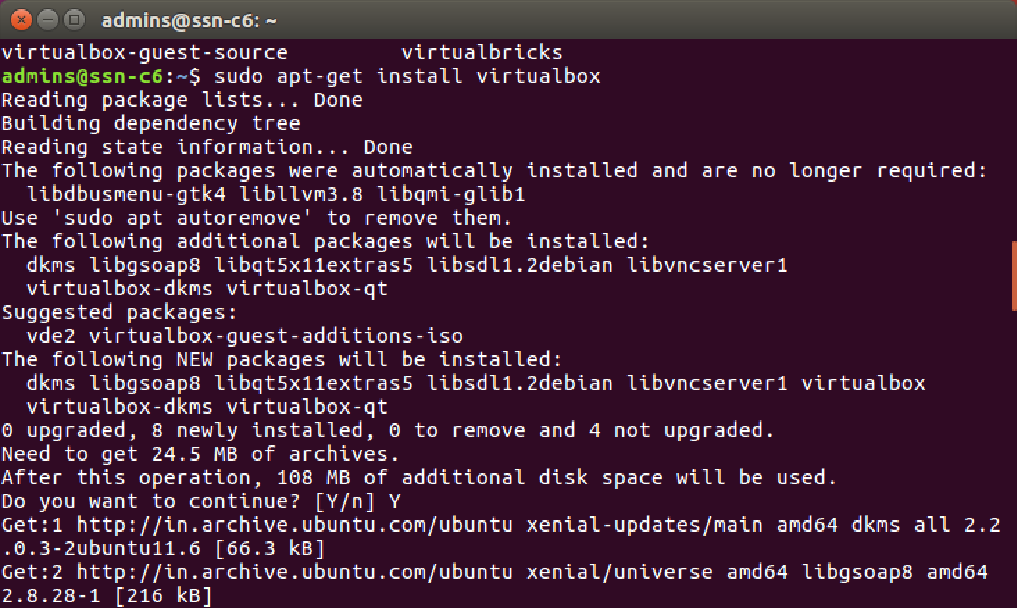
\includegraphics[scale=0.30,center]{fig1.png}
	\caption{Installing oracle virtualbox in native OS.}
	\label{fig:1}
	
\end{figure}

\begin{figure}[h]
	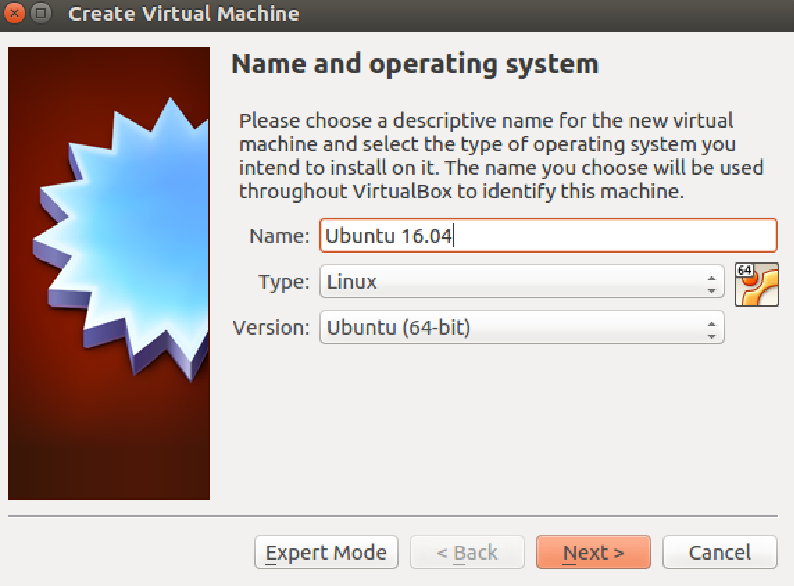
\includegraphics[scale=0.34,center]{fig2.png}
	\caption{Selecting the operating system flavour as Ubuntu 16.04 in guest OS instance.}
	\label{fig:2}
\end{figure}

\begin{figure}[h]
	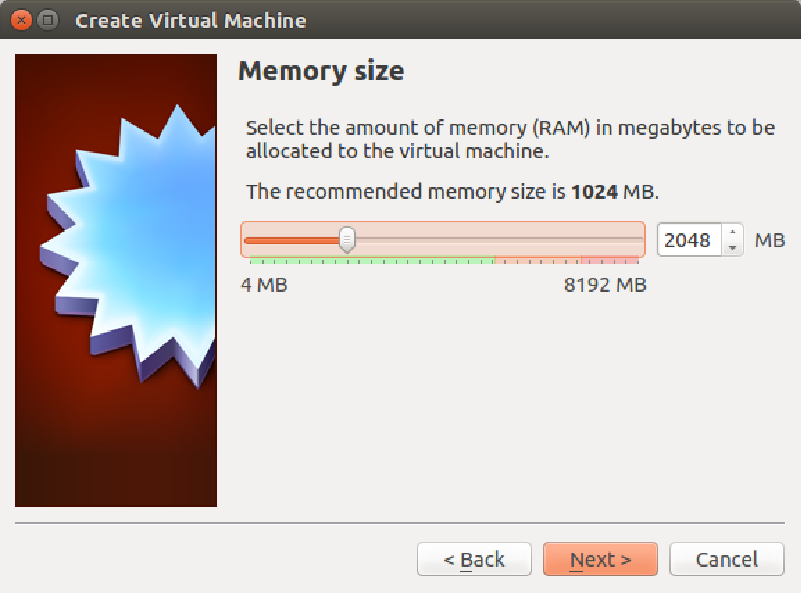
\includegraphics[scale=0.34,center]{fig3.png}
	\caption{Selecting the required RAM memory space for the VM instance.}
	\label{fig:3}
\end{figure}

\newpage
\begin{figure}[h]
	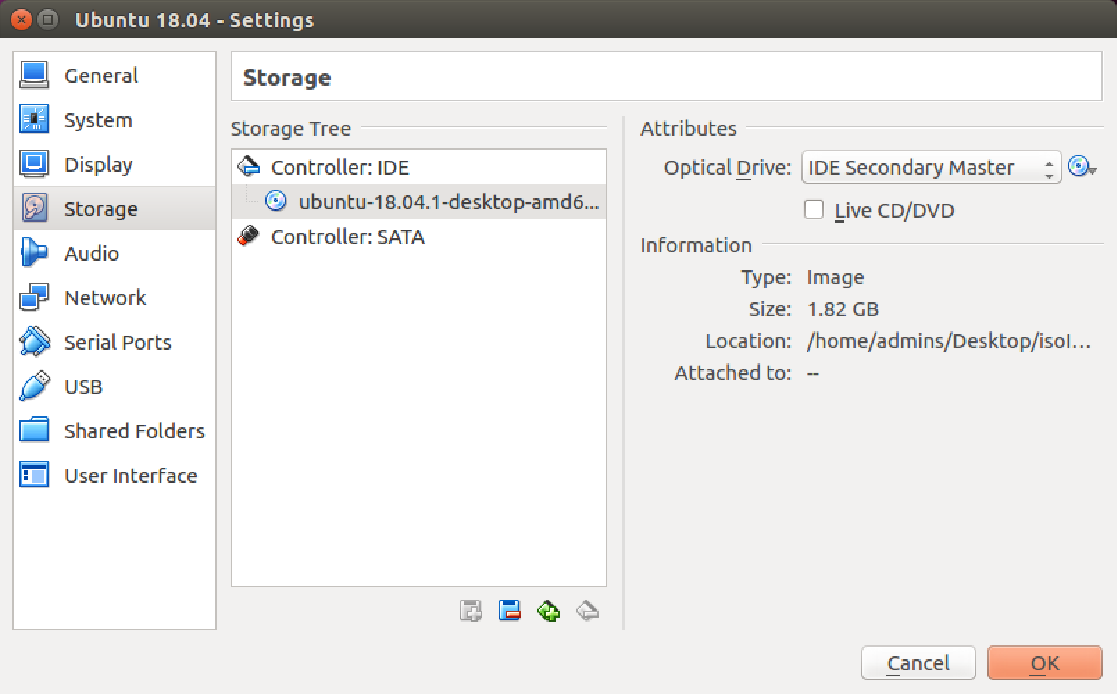
\includegraphics[scale=0.28,center]{fig4.png}
	\caption{Mounting the iso image as virtual hard disk drive to boot the guest OS.}
	\label{fig:4}
\end{figure}

\begin{figure}[h]
	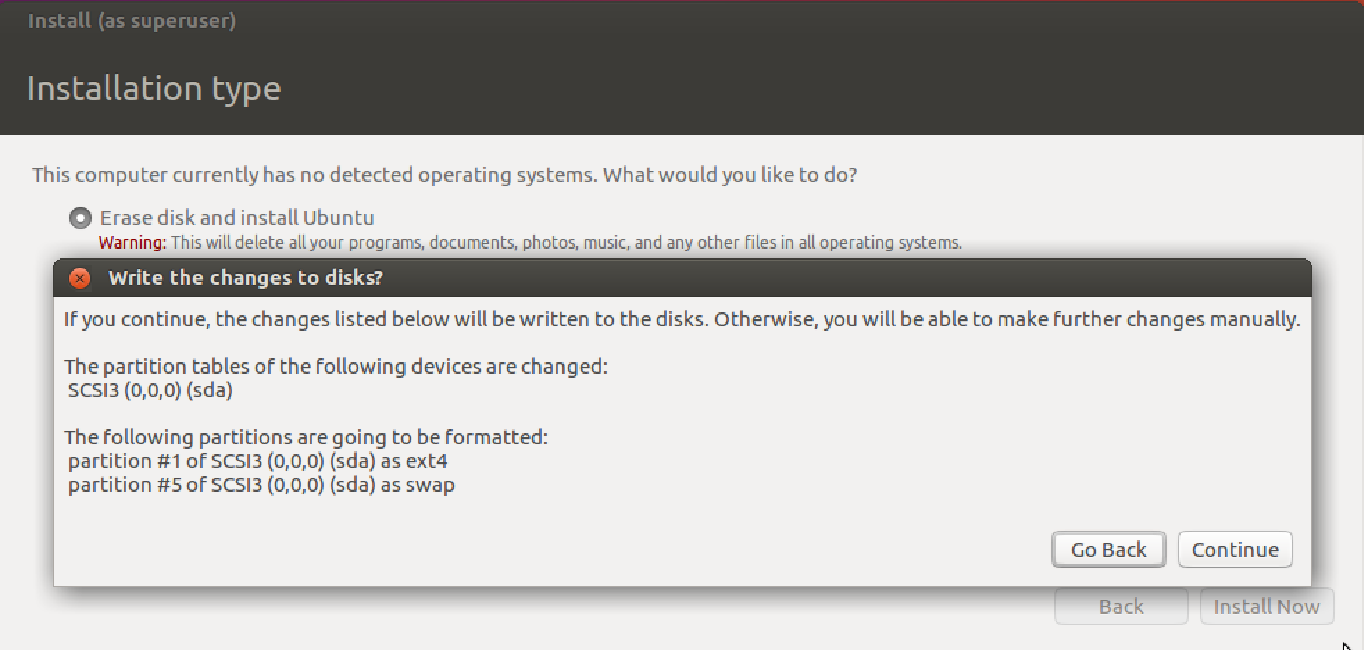
\includegraphics[scale=0.28,center]{fig5.png}
	\caption{Erase the hard disk and install Ubuntu 16.04.}
	\label{fig:5}
\end{figure}

\begin{figure}[h]
	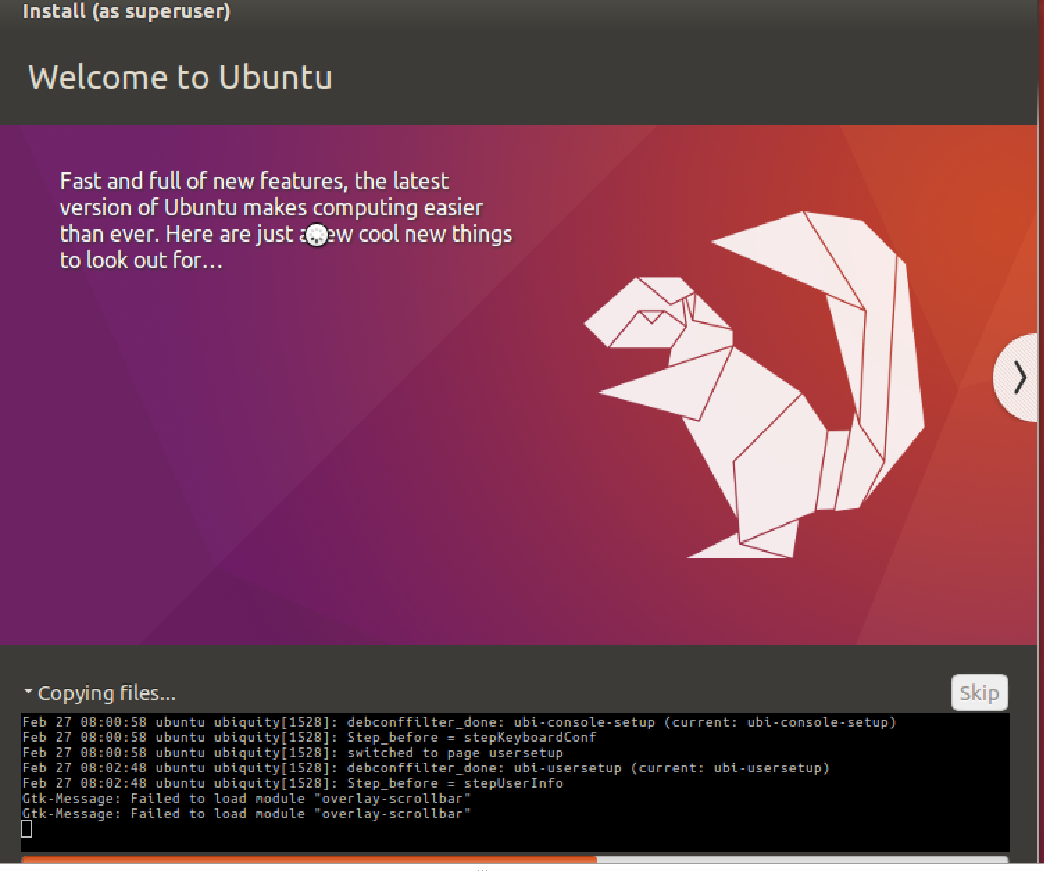
\includegraphics[scale=0.25,center]{fig6.png}
	\caption{Wait until all packages are installed in the new guest OS machine.}
	\label{fig:6}
\end{figure}

\newpage
\begin{figure}[h]
	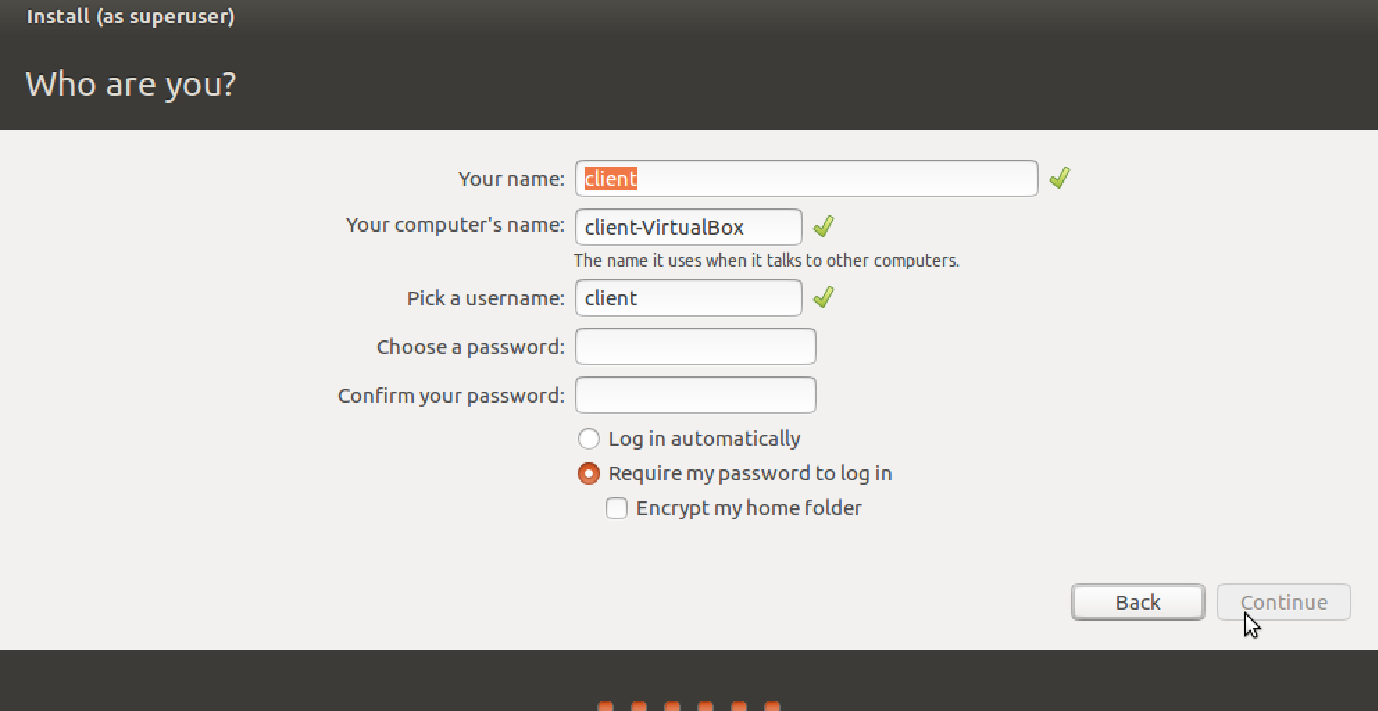
\includegraphics[scale=0.28,center]{fig7.png}
	\caption{Create new user with appropriate credentials.}
	\label{fig:7}
\end{figure}

	\begin{figure}[h]
		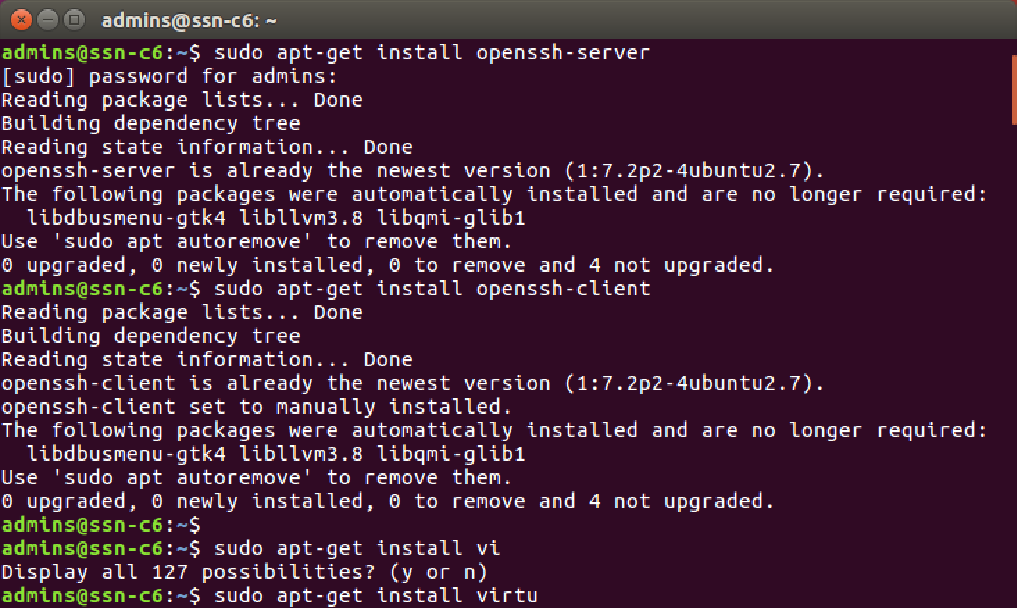
\includegraphics[scale=0.28,center]{fig8.png}
		\caption{Install required packages in the created virtual instance.}
		\label{fig:8}
	\end{figure}

\section{Result}
Thus the oracle virtualbox VM instance is sucessfully created with Ubuntu 16.04 OS version and required packages are installed.

\end{document}
